\documentclass[letterpaper,12pt]{report}

\usepackage[english]{babel}
\usepackage[utf8]{inputenc}
\usepackage{amsmath}
\usepackage{graphicx}
\usepackage[top=1in, bottom=1in, left=1.5in, right=1in]{geometry}
\usepackage[doublespacing]{setspace}
\usepackage{titlesec}

\title{Vortex Dominated Flows: A High-Order, Conservative Eulerian Simulation Method}

\author{Josh Bevan}

\date{\today}

\titleformat{\section}{\large\bfseries}{\thesection}{1em}{}
\titleformat{\subsection}{\normalsize\bfseries}{\thesection}{1em}{}

\begin{document}
\maketitle
%------------------------------------
\begin{abstract}
A high-order, conservative Eulerian method is presented for the simulation of vortex dominated inviscid fluid flows. The primitive variable Navier-Stokes equations are recast in the velocity-vorticity form to explicitly enforce conservation of vorticity. The advection of the vorticity is then calculated via a two-step process each time-step: the velocity field is determined by evaluation of the Biot-Savart integral, and then a line-based discontinuous Galerkin (DG) Eulerian spatial discretization scheme is applied. The accuracy and convergence of this method is examined for test cases where an analytical solution exists, as well as more challenging test cases which lack an analytical solution. Of particular interest is the influence the discretization of the calculated velocity field has on the performance of the method.
\end{abstract}

%------------------------------------
\section{Introduction}
\subsection{Problem Formulation}
-DNS expensive \\
-For inviscid vortex dominated flows $\rightarrow$ reformulate from primitive variables to velocity-vorticity \\
-Existing methods: Lagrangian vortex particle methods [Carley, Strain, Leonard] and VTM [Brown]\\
-Difficulty extending to high order: Particle methods (re-meshing), VTM (extended stencil)\\
-Available high order methods unsuitable: FD/FV (extended stencil and smearing), FE (non-conservative, ill-suited for hyperbolic), Spectral (Globally defined vs concentrated sparse vorticity)
\subsection{Chosen Methods}
-DG: conservative, local, flux funs handle hyperbolicity\\
-Line DG easy implementation for hexahedral meshes. Tensor product points allow possibility of easy biasing along principal flow directions. Allow easy translation of 1D methods for multidimensional domains\\
-Direct evaluation of BS integral: allows investigation of local order refinement effects on global convergence
\subsection{Thesis Structure}
-Theory: Develop method specific mathematics (DG, VTM, BS, etc)\\
-Methodology: Cover relevant notable implementation specifics (e.g. Solver structure, non-trivial algorithms), present convergence test structure (analytical cases, elliptical blob, 2-D "ring",several interacting patches) vs (convergence rate of: constant order velocity field, linear far field velocity [far= 1 element or X element separation], variable far field velocity order [heuristic?])\\
-Results: Results of matrix of tests (summary with aggregate plots, and selected results)\\
-Discussion: Analytical validation, comparison of velocity field fidelity test, comments on effects of global convergence

%------------------------------------
\section{Theory}
\subsection{Navier-Stokes: Velocity-vorticity form}
Quick derivation
\subsection{Discontinuous Galerkin}
Derivation with expansion on non-linear flux, salient points from line-DG
\subsection{Velocity Field Evaluation: The Biot-Savart Integral}
Expense of calculation (\% of total program?), Self-terms: Subsplitting vs GL quadrature skip vs kernels
\section{Methodology}
\subsection{Overall Solver Structure}
IC and BC initialization, Lagrange pre-calculation, mass and stiffness matrices generation, 2 step spatial discretization, time discretization, post processing
\subsection{Algorithms of Note}
Vectorized Lagrange evaluation, Lagrange derivatives, etc
\subsection{Validation and Convergence of Proposed Methods}
(analytical cases, elliptical blob, 2-D "ring",several interacting patches) vs (convergence rate of: constant order velocity field, linear far field velocity [far= 1 element or X element separation], variable far field velocity order [heuristic?])
\section{Results}
\subsection{Analytical Test Cases}
\subsection{Elliptical Blob}
\subsection{Arbitrary Patch}
\subsection{Dipole(misuse of term?)}
\subsection{Vortical System}
\section{Discussion}
\subsection{Analytical Validation of Model}
Comparison of existing analytical solutions vs model (Euler vortex, 5th order poly, other Saffmann test cases)
\subsection{}
\section{Conclusion}
\subsection{Weak Formulation}
\section{Recommendations}
\subsection{Weak Formulation}
\section{Literature Cited}
\begin{figure}
\centering
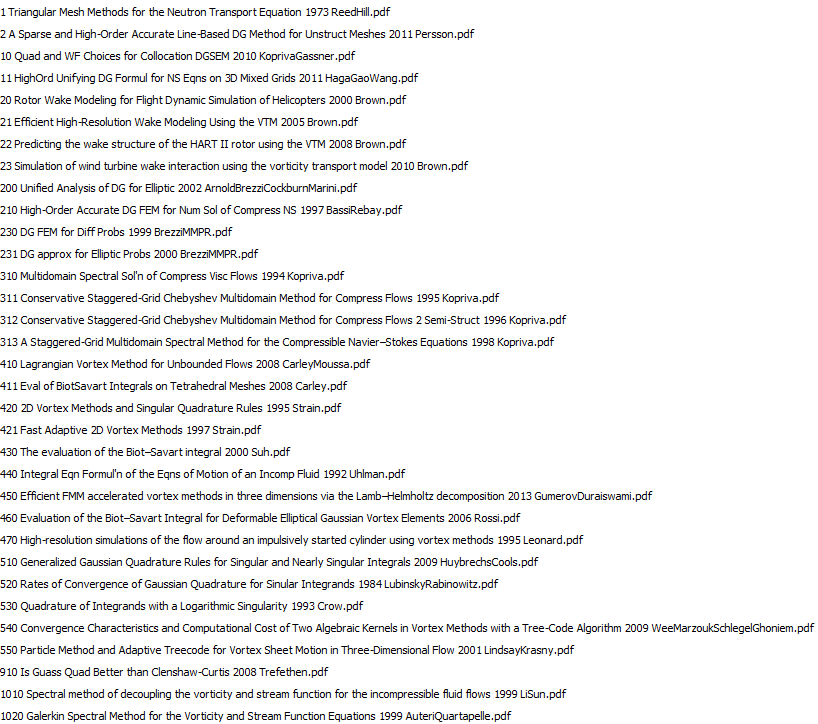
\includegraphics[width=1.4\textwidth]{LitStart.PNG}
\caption{\label{fig:ring}Dirty preliminary lit cited.}
\end{figure}

\end{document}